% !TeX root = surprises.tex

\chapter{Ramsey Theory}\label{c.ramsey}

%%%%%%%%%%%%%%%%%%%%%%%%%%%%%%%%%%%%%%%%%%%%%%%%%%%%%%%%%%%

Die Ramsey-Theorie ist ein Teilgebiet der Kombinatorik, das Fragen der folgenden Art stellt: Wie groß muss eine Menge sein, damit, wenn sie in Teilmengen unterteilt wird, mindestens eine Teilmenge eine bestimmte Eigenschaft hat?
Die Ergebnisse der Ramsey-Theorie sind schwer zu beweisen, und es bleiben viele Probleme offen. In diesem Kapitel stellen wir einfache Fälle von vier Problemen vor, um einen Eindruck von diesem faszinierenden Thema zu vermitteln: Schur-Dreier (Sect.~\ref{s.schur})---Dreier von ganzen Zahlen, so dass $a+b=c$, Pythagoras-Dreier (Sect.~\ref{s.pyth})---Dreier von ganzen Zahlen, so dass $a^2+b^2=c^2$, van der Waarden's Problem (Sect. ~\ref{s.van}), das Zahlenfolgen betrifft, und Ramsey's Theorem (Sect.~\ref{s.ramsey}) über die Färbung von Graphen. Abschnitt~\ref{s.bounds} zeigt, wie die probabilistische Methode in der Kombinatorik verwendet werden kann, um eine untere Schranke für Ramsey-Zahlen zu entwickeln.

Das Problem der pythagoräischen Tripel wurde kürzlich mit Hilfe von Computern gelöst, und zwar mit einer relativ neuen Methode, dem so genannten SAT-Solving. Für Leser, die mit der Aussagenlogik vertraut sind, gibt Abschnitt ~\ref{s.sat} einen Überblick darüber, wie dies geschieht.

Abschnitt~\ref{s.plimpton} beschreibt die pythagoreischen Tripel, wie sie den Babyloniern vor viertausend Jahren bekannt waren.

Terminologie: \emph{monochromatisch} bedeutet \emph{mit der gleichen Farbe}.

%%%%%%%%%%%%%%%%%%%%%%%%%%%%%%%%%%%%%%%%%%%%%%%%%%%%%%%%%%%
\section{Schur Tripel}\label{s.schur}


\begin{definition}
Gegeben ist eine \emph{beliebige} Zerlegung der Menge der positiven ganzen Zahlen:
\[
S(n)=\{1,\ldots,n\}
\]
in zwei disjunkte Teilmengen $S_1,S_2$, gibt es $\{a,b,c\}\subseteq S_1$ oder $\{a,b,c\}\subseteq S_2$ (oder beide), so dass $a\!<\!b\!<\!c$ und $a+b=c$? Wenn ja, heißt die Menge $\{a,b,c\}$ ein \emph{Schur-Tripel}.
\end{definition}

\begin{example} Für $n=8$, in der Zersetzung:
\begin{align}
S_1 = \{1,2,3,4\},\; S_2 = \{5,6,7,8\}\,,
\label{eq.schur0}
\end{align}
die Menge $S_1$ enthält das Schur-Tripel $\{1,2,3\}$.
Allerdings ist die Zerlegung:
\begin{align}
S'_1 = \{1,2,4,8\},\; S'_2 = \{3,5,6,7\}\,,
\label{eq:schur1}
\end{align}
enthält kein Schur-Tripel, wie man durch Aufzählung aller Tripel in jeder Teilmenge überprüfen kann.
\end{example}

\begin{theorem}
In alle Zerlegungen von $S(9)=\{1,\ldots,9\}$ in zwei disjunkte Teilmengen, enthält mindestens eine Teilmenge ein Schur-Tripel.
\end{theorem}
Natürlich könnten wir die $2^9=512$ Zerlegungen von $S(9)$ in zwei disjunkte Teilmengen überprüfen, aber wir wollen versuchen, einen prägnanteren Beweis zu finden.
\begin{proof}
Wir versuchen, eine Zerlegung zu konstruieren, die kein Schur-Tripel enthält, und zeigen, dass dies aufgrund der Nebenbedingungen des Problems unmöglich ist. Wir beginnen damit, $1$ und $3$ in die Teilmenge $S_1$ zu legen. $2$ muss in $S_2$ liegen, weil $1+2=3$ und wir versuchen, eine Zerlegung zu konstruieren, die kein Schur-Tripel enthält. Ähnlich muss $4$ in $S_2$ liegen, weil $1+3=4$. Weiter, $6$ kommt in $S_1$, weil $2+4=6$ und $7$ kommt in $S_2$, weil $1+6=7$. Aber $3+6=9$ und $2+7=9$, also muss $9$ sowohl in $S_1$ als auch in $S_2$ vorkommen, ein Widerspruch. Die Reihenfolge der Schlussfolgerungen ist in der folgenden Tabelle dargestellt:
\[
\begin{array}{l@{\hspace{2em}}l}
S_1&S_2\\\hline
1,3 & \\
1,3 & 2\\
1,3 & 2,4\\
1,3,6 & 2,4\\
1,3,6 & 2,4,7\\
1,3,6,9 & 2,4,7\\
1,3,6,9 & 2,4,7,9
\end{array}
\]
Zurückverfolgend suchen wir nach einer Zerlegung, bei der $1,3$ in verschiedenen Teilmengen liegen. Wenn wir $5$ in $S_2$ unterbringen, führt eine Folge von Schlussfolgerungen wieder zu einem Widerspruch, weil $9$ in beiden Teilmengen vorkommen muss. Der Leser soll jede der in der folgenden Tabelle aufgeführten Schlüsse begründen:
\[
\begin{array}{l@{\hspace{2em}}l}
S_1&S_2\\\hline
1&3\\
1 & 3,5\\
1,2&3,5\\
1,2,8&3,5\\
1,2,8&3,5,7\\
1,2,8&3,5,7,9\\
1,2,8&3,5,6,7,9\\
1,2,8,9&3,5,6,7,9
\end{array}
\]
Wir gehen wieder zurück und versuchen, $5$ in $S_1$ zu platzieren, aber auch das führt zu einem Widerspruch, wie die folgende Tabelle zeigt:
\[
\begin{array}{l@{\hspace{2em}}l}
S_1&S_2\\\hline
1&3\\
1,5& 3\\
1,5&3,4\\
1,5&3,4,6\\
1,2,5&3,4,6\\
1,2,5&3,4,6,7\\
1,2,5,7&3,4,6,7
\end{array}
\]
Daraus folgt, dass es keine Zerlegung gibt, die nicht ein Schur-Tripel enthält.
\end{proof}
Issai Schur bewies das folgende Theorem:
\begin{theorem}[Schur]
Für jedes $k\geq 2$ gibt es ein kleinstes $n$, so dass in jeder disjunkten Zerlegung von $S(n)$ in $k$ Teilmengen mindestens eine der Teilmengen ein Schur-Tripel enthalten muss.
\end{theorem}

%%%%%%%%%%%%%%%%%%%%%%%%%%%%%%%%%%%%%%%%%%%%%%%%%%%%%%%%%%%

\section{Pythagoräische Dreiergruppen}\label{s.pyth}

\begin{definition}
Gegebene \emph{beliebige} Zerlegung der Menge der positiven ganzen Zahlen:
\[
S(n)=\{1,\ldots,n\}
\]
in zwei disjunkte Teilmengen $S_1,S_2$, gibt es $\{a,b,c\}\subseteq S_1$ oder $\{a,b,c\}\subseteq S_2$ (oder beide), so dass $a\!<\!b\!<\!c$ und $a^2+b^2=c^2$? Wenn ja, wird $\{a,b,c\}$ ein \emph{Pythagoreisches Tripel} genannt.
\end{definition}

\begin{example}
Für $n=10$, bei der Zerlegung in gerade und ungerade Zahlen:
\[
S_1 = \{1,3,5,7,9\},\; S_2=\{2,4,6,8,10\}\,,
\]
es gibt keine pythagoreischen Tripel in $S_1$, aber $\{6,8,10\}$ in $S_2$ ist ein pythagoreisches Tripel, da $6^2+8^2=10^2$.
\end{example}

Marijn J.H. Heule und Oliver Kullmann bewiesen die folgenden Theoreme. Ihre Beweismethode wird in Abschnitt ~\ref{s.sat} diskutiert.

\begin{theorem}
Für alle $n\leq 7824$ gibt es \emph{eine} Zerlegung von $S(n)$ in zwei disjunkte Teilmengen, so dass beide Teilmengen \emph{kein} pythagoreisches Tripel enthalten.
\end{theorem}

\begin{theorem}
Für alle $n\leq 7824$ gibt es \emph{irgendeine} Zerlegung von $S(n)$ in zwei disjunkte Teilmengen, so dass beide Teilmengen \emph{kein} pythagoreisches Tripel enthalten.
\end{theorem}
Es ist unmöglich, alle $2^{7825}$-Zerlegungen von $S(7825)$ zu prüfen. Wenn wir jede Mikrosekunde eine Zerlegung prüfen könnten, ergäbe das $2^{7825}\; \textrm{microseconds}\approx 10^{600}\; \textrm{years}$, während das geschätzte Alter des Universums nur etwa $10^{10}$ Jahre beträgt.

%%%%%%%%%%%%%%%%%%%%%%%%%%%%%%%%%%%%%%%%%%%%%%%%%%%%%%%%%%%

\section{Das Problem von Van der Waerden}\label{s.van}

Betrachten Sie die Sequenzen von acht farbigen Punkten in Abb.~\ref{f.vdw1}. In der oberen Folge befinden sich rote Punkte an den Positionen $(1,2,3)$ und blaue Punkte an den Positionen $(4,5,6)$. In jedem Fall bilden die Positionen eine arithmetische Progression. Auch in der mittleren Folge bilden die roten Punkte an den Positionen $(1,3,5)$ eine arithmetische Folge. In der unteren Folge gibt es jedoch keine Menge von drei einfarbigen Punkten, deren Positionen eine arithmetische Folge bilden. 
Dreiergruppen roter Punkte befinden sich an den Positionen $(1,2,5)$, $(1,2,6)$, $(2,5,6)$, von denen keine eine arithmetische Progression bildet, und ähnliches gilt für die blauen Punkte.

\begin{figure}[htb]
\begin{center}
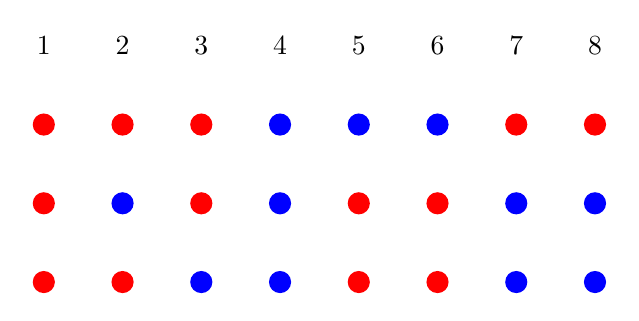
\begin{tikzpicture}
\foreach \x in {1,2,3,4,5,6,7,8} {
  \node at (\x,3) {$\x$};
}
\foreach \x/\col in {1/red,2/red,3/red,4/blue,5/blue,6/blue,7/red,8/red} {
  \fill[\col] (\x,2) circle(4pt);
}
\foreach \x/\col in {1/red,2/blue,3/red,4/blue,5/red,6/red,7/blue,8/blue} {
  \fill[\col] (\x,1) circle(4pt);
}
\foreach \x/\col in {1/red,2/red,3/blue,4/blue,5/red,6/red,7/blue,8/blue} {
  \fill[\col] (\x,0) circle(4pt);
}
\end{tikzpicture}
\end{center}
\caption{van der Waerden's Problem für acht farbige Punkte}\label{f.vdw1}
\end{figure}

Bei neun Punkten muss jede Färbung eine Folge von drei monochromen Punkten enthalten, die eine arithmetische Progression bilden. Fügen wir zum Beispiel einen roten oder einen blauen Punkt am Ende der unteren Folge in Abb.~\ref{f.vdw1} hinzu, so erhalten wir die Folgen in Abb.~\ref{f.vdw2}. In der oberen Folge gibt es rote Punkte an den Positionen $(1,5,9)$, eine arithmetische Progression, und in der unteren Folge gibt es blaue Punkte an den Positionen $(7,8,9)$, ebenfalls eine arithmetische Progression.
\begin{figure}[htb]
\begin{center}
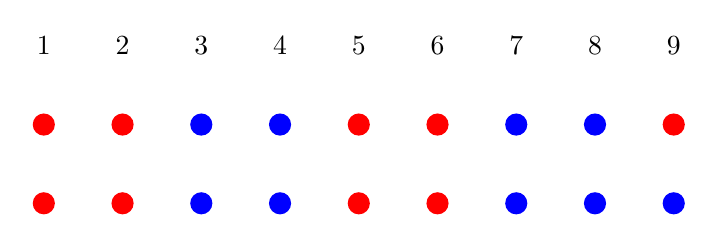
\begin{tikzpicture}
\foreach \x in {1,2,3,4,5,6,7,8,9} {
  \node at (\x,2) {$\x$};
}
\foreach \x/\col in {1/red,2/red,3/blue,4/blue,5/red,6/red,7/blue,8/blue,9/red} {
  \fill[\col] (\x,1) circle(4pt);
}
\foreach \x/\col in {1/red,2/red,3/blue,4/blue,5/red,6/red,7/blue,8/blue,9/blue} {
  \fill[\col] (\x,0) circle(4pt);
}
\end{tikzpicture}
\end{center}
\caption{van der Waerden's Problem für neun farbige Punkte}\label{f.vdw2}
\end{figure}
Bartel L. van der Waerden stellte das folgende Problem: Für jede positive ganze Zahl $k$, was ist die kleinste Zahl $n$, so dass \emph{jede} Folge von $n$ farbigen Punkten \emph{muss} eine Folge von $k$ monochromatischen Punkten enthalten, die eine arithmetische Progression bilden? Für $k=3$, $n=9$, wie oben für eine Zerlegung gezeigt. Das nächste Ergebnis ist schwieriger zu zeigen: für $k=4$, $n=35$.


%%%%%%%%%%%%%%%%%%%%%%%%%%%%%%%%%%%%%%%%%%%%%%%%%%%%%%%%%%%


\section{Ramsey's Theorem}\label{s.ramsey}

Färben Sie die Kanten von $K_5$, dem vollständigen Graphen mit $5$ Scheitelpunkten, mit zwei Farben wie in Abb.~\ref{f.ramsey5} gezeigt. Es gibt keine einfarbigen Untergraphen $K_3$ (Dreiecke) in dem Graphen. Abbildung~\ref{f.ramsey6} zeigt eine Färbung von $K_6$ und es ist leicht zu sehen, dass es monochromatische Dreiecke $\triangle ACE$ und $\triangle BDF$ gibt. In diesem Abschnitt beweisen wir einen einfachen Fall eines Theorems von Frank P. Ramsey über die Existenz von Teilmengen mit einer bestimmten Eigenschaft.
\begin{figure}[ht]
\subfigures
\leftfigure[c]{
\begin{tikzpicture}
\node (pentagon) [minimum size=5cm,regular polygon,regular polygon sides=5] at (0,0) {};
\draw[red]  (pentagon.corner 1) node[black,above] {$A$} -- (pentagon.corner 2);
\draw[red]  (pentagon.corner 2) node[black,left] {$B$} -- (pentagon.corner 3);
\draw[red]  (pentagon.corner 3) node[black,left] {$C$} -- (pentagon.corner 4);
\draw[red]  (pentagon.corner 4) node[black,right] {$D$} -- (pentagon.corner 5);
\draw[red]  (pentagon.corner 5) node[black,right] {$E$} -- (pentagon.corner 1);
\draw[dashed,blue] (pentagon.corner 1) -- (pentagon.corner 3);
\draw[dashed,blue] (pentagon.corner 1) -- (pentagon.corner 4);
\draw[dashed,blue] (pentagon.corner 2) -- (pentagon.corner 4);
\draw[dashed,blue] (pentagon.corner 2) -- (pentagon.corner 5);
\draw[dashed,blue] (pentagon.corner 3) -- (pentagon.corner 5);
\end{tikzpicture}
}
\hfill
\rightfigure[c]{
\begin{tikzpicture}
\node (hexagon) [minimum size=5cm,regular polygon,regular polygon sides=6] at (0,0) {};
\draw[red]  (hexagon.corner 1) node[black,above] {$A$} -- (hexagon.corner 2);
\draw[red]  (hexagon.corner 2) node[black,above] {$B$} -- (hexagon.corner 3);
\draw[red]  (hexagon.corner 3) node[black,left] {$C$} -- (hexagon.corner 4);
\draw[red]  (hexagon.corner 4) node[black,left] {$D$} -- (hexagon.corner 5);
\draw[red]  (hexagon.corner 5) node[black,right] {$E$} -- (hexagon.corner 6);
\draw[red]  (hexagon.corner 6) node[black,right] {$F$} -- (hexagon.corner 1);
\draw[dashed,blue] (hexagon.corner 1) -- (hexagon.corner 3);
\draw[dashed,blue] (hexagon.corner 1) -- (hexagon.corner 4);
\draw[dashed,blue] (hexagon.corner 1) -- (hexagon.corner 5);
\draw[dashed,blue] (hexagon.corner 2) -- (hexagon.corner 4);
\draw[dashed,blue] (hexagon.corner 2) -- (hexagon.corner 5);
\draw[dashed,blue] (hexagon.corner 2) -- (hexagon.corner 6);
\draw[dashed,blue] (hexagon.corner 3) -- (hexagon.corner 5);
\draw[dashed,blue] (hexagon.corner 3) -- (hexagon.corner 6);
\draw[dashed,blue] (hexagon.corner 4) -- (hexagon.corner 6);
\end{tikzpicture}
}
\leftcaption{Eine Färbung von $K_5$ mit zwei Farben}\label{f.ramsey5}
\rightcaption{Eine Färbung $K_6$ mit zwei Farben}\label{f.ramsey6}
\end{figure}
\begin{definition}
$\quad R(k)$, die \emph{Ramsey-Zahl} für $k$, ist die kleinste Zahl $n$, so dass in \emph{jeder} Färbung von $K_{n}$, dem vollständigen Graphen auf $n$ Scheitelpunkten, mit zwei Farben ein monochromatischer vollständiger Teilgraph $K_k$ existiert.
\end{definition}

\begin{theorem}[Ramsey]
$\quad R(3)=6$.\label{thm.ramsey}
\end{theorem}

\begin{proof}

Abbildung~\ref{f.ramsey5} zeigt, dass $R(3)>5$. Um zu zeigen, dass $R(3)\leq 6$ ist, betrachtet man einen beliebigen Knoten $v$ in $K_6$. $v$ ist mit fünf anderen Knoten verbunden, und wenn die Kanten mit zwei Farben gefärbt sind, muss es mindestens drei einfarbige Kanten geben, die mit $v$ verbunden sind. 

In Abb.~\ref{f.ramsey4a} sind $\overline{AB}, \overline{AC}, \overline{AE}$ rot gefärbt. Da der Graph vollständig ist, sind alle Eckpunkte miteinander verbunden. Wenn also eine der Kanten $\overline{BC}$, $\overline{BE}$, $\overline{CE}$ rot gefärbt ist, sagen wir $\overline{BE}$, wird ein rotes Dreieck $\triangle ABE$ gebildet. Andernfalls sind alle drei Kanten dieser Kanten blau gefärbt und sie bilden ein blaues Dreieck (Abb.~\ref{f.ramsey4b}).
\end{proof}

Das Theorem kann auf eine beliebige Anzahl von Farben verallgemeinert werden, sowie auf Färbungen, bei denen die Größen der Untergraphen nicht gleich sind. $R(r,b,g)$ ist der kleinste vollständige Graph, der so beschaffen ist, dass in jeder Färbung mit drei Farben vollständige Teilgraphen mit $r$ roten Kanten, $b$ blauen Kanten und $g$ grünen Kanten existieren müssen.

\begin{figure}[hb]
\subfigures
\leftfigure[c]{
\begin{tikzpicture}
\node (hexagon) [minimum size=5cm,regular polygon,regular polygon sides=6] at (0,0) {};
\draw[red]  (hexagon.corner 1) node[black,above] {$A$} -- (hexagon.corner 2) node[black,above] {$B$};
\draw[blue,dashed]  (hexagon.corner 1) -- (hexagon.corner 6) node[black,right] {$F$};
\draw[red] (hexagon.corner 1) -- (hexagon.corner 3) node[black,below] {$C$};
\draw[blue,dashed] (hexagon.corner 1) -- (hexagon.corner 4) node[black,right] {$D$};
\draw[red] (hexagon.corner 1) -- (hexagon.corner 5) node[black,right] {$E$};
\end{tikzpicture}
}
\hfill
\rightfigure[c]{
\begin{tikzpicture}
\node (hexagon) [minimum size=5cm,regular polygon,regular polygon sides=6] at (0,0) {};
\draw[very thick,red]  (hexagon.corner 1) node[black,above] {$A$} -- (hexagon.corner 2) node[black,above] {$B$};
\draw[blue,dashed]  (hexagon.corner 1) -- (hexagon.corner 6) node[black,right] {$F$};
\draw[red] (hexagon.corner 1) -- (hexagon.corner 3) node[black,below] {$C$};
\draw[blue,dashed] (hexagon.corner 1) -- (hexagon.corner 4) node[black,right] {$D$};
\draw[very thick,red] (hexagon.corner 1) -- (hexagon.corner 5) node[black,right] {$E$};
\draw[very thick,red] (hexagon.corner 2) -- (hexagon.corner 5);
\draw[very thick,blue,dashed] (hexagon.corner 2) -- (hexagon.corner 3);
\draw[very thick,blue,dashed] ($(hexagon.corner 2)+(-2pt,0)$) -- ($(hexagon.corner 5)+(-2pt,0)$);
\draw[very thick,blue,dashed] (hexagon.corner 5) -- (hexagon.corner 3);
\end{tikzpicture}
}
\leftcaption{Ein Scheitelpunkt von $K_6$}\label{f.ramsey4a}
\rightcaption{Monochromatische Dreiecke in $K_6$}\label{f.ramsey4b}
\end{figure}

%%%%%%%%%%%%%%%%%%%%%%%%%%%%%%%%%%%%%%%%%%%%%%%%%%%%%%%%%%%

\section{Die probabilistische Methode}\label{s.bounds}

Die einzigen bekannten nicht-trivialen Ramsey-Zahlen sind $R(3)=6$ und $R(4)=18$. 1947 entwickelte Paul Erd\H{o}ss die \emph{probabilistische Methode} und verwendete sie, um untere und obere Schranken für $R(k)$ zu zeigen. Spätere Forschungen haben beide Schranken verbessert, aber dies ist immer noch ein wichtiges Forschungsgebiet, da die Schranken nicht eng sind. Es wurde zum Beispiel bewiesen, dass $43\leq R(5) \leq 48$ und $798\leq R(10)\leq 23556$. In diesem Abschnitt wird die Elementarwahrscheinlichkeit verwendet, um eine untere Schranke für $R(k)$ zu erhalten.

Um zu zeigen, dass es ein Element einer Menge $S$ gibt, das die Eigenschaft $A$ besitzt, muss man beweisen, dass die Wahrscheinlichkeit, dass ein \emph{zufälliges} Element von $S$ die Eigenschaft $A$ besitzt, größer als Null ist. Es ist wichtig zu verstehen, dass die Methode \emph{nicht-konstruktiv} ist: Sie beweist nur, dass ein solches Element existiert, konstruiert es aber nicht. Obwohl wir aus Thm.~\ref{thm.ramsey} wissen, dass $R(3)=6$ ist, wollen wir die probabilistische Methode verwenden, um eine untere Schranke für $R(3)$ zu erhalten.

\begin{theorem}[Erd\H{o}s]
$\quad R(3) > 4$.
\end{theorem}
\begin{proof}
Betrachten Sie bei einer \emph{zufälligen} Färbung von $K_n$ durch die beiden Farben Rot und Blau einen beliebigen Untergraphen $K_3$, d.h. ein beliebiges Dreieck mit $\binom{3}{2}=3$ Seiten. Die Wahrscheinlichkeit, dass alle Seiten rot gefärbt sind, ist $2^{-3}$, ebenso die Wahrscheinlichkeit, dass alle Seiten blau gefärbt sind, also ist die Wahrscheinlichkeit, dass das Dreieck einfarbig ist, $2^{-3}+2^{-3}=2^{-2}=1/4$. Die Anzahl der Dreiecke in $K_n$ ist $\binom{n}{3}$, also ist $P(n,3)$, die Wahrscheinlichkeit, dass $\emph{irgendein}$ Dreieck, das in einer zufälligen Färbung von $K_n$ enthalten ist, einfarbig ist, gleich:
\[
P(n,3)=\binom{n}{3}\cdot \frac{1}{4}\,.
\]
Wenn $P(n,3)<1$, dann ist sein Komplement $\overline{P}(n,3)=1-P>0$, d.h. die Wahrscheinlichkeit, dass eine zufällige Färbung von $K_n$ kein monochromatisches Dreieck enthält, ist größer als Null, also muss mindestens eines existieren.

Die folgende Tabelle zeigt $\overline{P}(n,3)$ für verschiedene Werte von $n$, und ob der Wert von $\overline{P}(n,3)$ beweist, dass es eine Färbung ohne einfarbiges Dreieck gibt:
\[
\renewcommand*{\arraystretch}{1.1}
\begin{array}{r@{\hspace{5mm}}r@{\hspace{5mm}}r}
\hline
\noalign{\smallskip}
n & \overline{P}(n,3) & \textit{Exists}\\
\noalign{\smallskip}\hline\noalign{\smallskip}
3 & 3/4 & \textit{yes} \\
4 & 5/6 & \textit{yes}\\
5 & -3/7 & \textrm{--}\\
\noalign{\smallskip}
 \hline
 \end{array}
\]
\end{proof}
Auf den ersten Blick ist das Ergebnis seltsam, denn Abb.~\ref{f.ramsey5} zeigt, dass es eine Färbung von $K_5$ ohne monochromatische Färbung gibt. Das probabilistische Kriterium ist jedoch hinreichend, aber nicht notwendig; es ist eine untere Schranke, was bedeutet, dass $R(n)>4$ ist, was wahr ist, weil Thm.~\ref{thm.ramsey} gezeigt hat, dass $R(n)=6$.

Der gleiche Beweis funktioniert für beliebige $k$, so dass die Wahrscheinlichkeit für die Existenz einer Färbung von $K_n$ ohne monochromatischen vollständigen Graphen $K_k$ ist:
\[
P(n,k)=\binom{n}{k}\cdot 2\cdot 2^{-\binom{k}{2}}\,.
\]
For $k=4$:
\begin{eqnarray*}
\overline{P}(n,4)&=&1-\binom{n}{4}\cdot 2^{-5}=\left.\left(32-\binom{n}{4}\right)\right/32\\
\overline{P}(6,4)&=&(32-15)/32=17/32\\
\overline{P}(7,4)&=&(32-35)/32=-3/32\,.
\end{eqnarray*}
Daraus folgt, dass $R(4)>6$ ist, was viel weniger ist als der bekannte Wert $R(4)=18$.

%%%%%%%%%%%%%%%%%%%%%%%%%%%%%%%%%%%%%%%%%%%%%%%%%%%%%%%%%%%

\section{SAT-Auflösung}\label{s.sat}

SAT-Solving ist eine Methode zur Lösung von Problemen, bei der ein Problem als Formel in der Aussagenlogik kodiert und dann mit einem Computerprogramm auf den Wahrheitswert der Formel überprüft wird. Fortschritte bei den Algorithmen und Implementierungen haben das SAT-Solving zu einem praktikablen Ansatz für die Problemlösung gemacht. Wir geben einen Überblick über das SAT-Solving und erklären, wie es zur Lösung der in diesem Kapitel beschriebenen mathematischen Probleme verwendet werden kann. Es wird vorausgesetzt, dass der Leser über elementare Kenntnisse der Aussagenlogik verfügt, wie sie in Def.~\ref{def.sat}. zusammengefasst sind.

\subsection{Propositionale Logik und das SAT-Problem}

\begin{definition}\label{def.sat}\mbox{}\\
\begin{itemize}
\item Eine \emph{Formel} besteht aus \emph{atomaren Formeln} oder \emph{Atomen}, die durch die propositionalen Operatoren $\vee$ (Disjunktion, ``oder''), $\wedge$ (Konjunktion, ``und''), $\neg$ (Negation, ``nicht'') verbunden sind.
\item Eine Formel erhält eine \emph{Interpretation} durch eine Zuordnung von $T$ oder $F$ zu jedem Atom. Die Auswertung einer Formel in einer Interpretation ergibt ihren \emph{Wahrheitswert} $T$ oder $F$. 
\item Eine Formel ist \emph{satisfiable}, wenn und nur wenn es eine Interpretation gibt, die ihren Wahrheitswert $T$ ergibt. Andernfalls ist die Formel \emph{unbefriedigend}.
\item Eine Formel ist dann und nur dann in \emph{conjunctive normal form (CNF)}, wenn sie aus einer Konjunktion von Teilformeln besteht, von denen jede eine Disjunktion von \emph{literals} (Atomen oder Negationen von Atomen) ist.
\end{itemize}
\end{definition}

Die folgende Formel ist in CNF:
\[
(\neg p \vee q \vee \neg \,r) \;\wedge\; (\neg p \vee r)
\;\wedge\; (\neg \,r)\;\wedge\;(p \vee q \vee \neg \,r)\,.
\]
Das \emph{SAT-Problem} besteht darin, zu entscheiden, ob eine gegebene Formel in CNF erfüllbar ist oder nicht. Ein \emph{SAT solver} ist ein Computerprogramm, das das SAT-Problem lösen kann. Die meisten SAT-Solver basieren auf dem DPLL-Algorithmus, der auf die 1960er Jahre zurückgeht, aber durch neuere Entwicklungen wurde der Algorithmus erheblich verbessert. Hochgradig optimierte Implementierungen dieser Algorithmen haben SAT-Solver zu einem wichtigen Werkzeug für die Lösung von Problemen in vielen Bereichen einschließlich der Mathematik gemacht.

\subsection{Schur-Tripel} Index {Schur-Tripel}

Wir kodieren das Schur-Tripel-Problem $S(8)$ als eine Formel in CNF. Die Formel ist dann und nur dann erfüllbar, wenn es eine Zerlegung der Menge $S$ in disjunkte Teilmengen $S_1,S_2$ gibt, so dass weder $S_1$ noch $S_2$ ein Schur-Tripel enthält. Für jede der Zahlen $1\leq i \leq 8$ gibt es ein Atom $p_i$. Die beabsichtigte Bedeutung einer Interpretation für die Formel ist, dass sie $p_i$ $T$ zuordnet, wenn $i$ in der ersten Teilmenge $S_1$ liegt, und sie ordnet $p_i$ $F$ zu, wenn $i$ in der zweiten Teilmenge $S_2$ liegt. Um zu zeigen, dass in allen Zerlegungen keine Teilmenge ein Schur-Tripel enthält, muss die Interpretation sicherstellen, dass für jedes mögliche Schur-Tripel mindestens ein Atom mit $T$ und ein Atom mit $F$ belegt ist. 

Zum Beispiel ist $\{2,4,6\}$ ein Schur-Tripel, so dass mindestens eine der drei ganzen Zahlen in $S_1$ und mindestens eine von ihnen in $S_2$ liegen muss. Daher muss $p_2 \vee p_4 \vee p_6$ wahr sein und auch $\neg p_2 \vee \neg p_4 \vee \neg p_6$ muss wahr sein. Es gibt $12$ mögliche Schur-Tripel, also lautet die CNF-Formel:
\begin{align}
\begin{array}{l}
(p_1 \vee p_2 \vee p_3) \;\wedge\; (\neg p_1 \vee \neg p_2 \vee \neg p_3) \;\wedge \\
(p_1 \vee p_3 \vee p_4) \;\wedge\; (\neg p_1 \vee \neg p_3 \vee \neg p_4) \;\wedge \\
(p_1 \vee p_4 \vee p_5) \;\wedge\; (\neg p_1 \vee \neg p_4 \vee \neg p_5) \;\wedge \\
(p_1 \vee p_5 \vee p_6) \;\wedge\; (\neg p_1 \vee \neg p_5 \vee \neg p_6) \;\wedge \\
(p_1 \vee p_6 \vee p_7) \;\wedge\; (\neg p_1 \vee \neg p_6 \vee \neg p_7) \;\wedge \\
(p_1 \vee p_7 \vee p_8) \;\wedge\; (\neg p_1 \vee \neg p_7 \vee \neg p_8) \;\wedge \\
(p_2 \vee p_3 \vee p_5) \;\wedge\; (\neg p_2 \vee \neg p_3 \vee \neg p_5) \;\wedge \\
(p_2 \vee p_4 \vee p_6) \;\wedge\; (\neg p_2 \vee \neg p_4 \vee \neg p_6) \;\wedge \\
(p_2 \vee p_5 \vee p_7) \;\wedge\; (\neg p_2 \vee \neg p_5 \vee \neg p_7) \;\wedge \\
(p_2 \vee p_6 \vee p_8) \;\wedge\; (\neg p_2 \vee \neg p_6 \vee \neg p_8) \;\wedge \\
(p_3 \vee p_4 \vee p_7) \;\wedge\; (\neg p_3 \vee \neg p_4 \vee \neg p_7) \;\wedge \\
(p_3 \vee p_5 \vee p_8) \;\wedge\; (\neg p_3 \vee \neg p_5 \vee \neg p_8)\,.
\end{array}\label{eq.schur2}
\end{align}
Wenn ein SAT-Solver diese Formel erhält, antwortet er, dass die Formel unter jeder der Interpretationen erfüllbar ist:
\[
\begin{array}{c@{\hspace{8pt}}c@{\hspace{8pt}}c@{\hspace{8pt}}c@{\hspace{8pt}}c@{\hspace{8pt}}c@{\hspace{8pt}}c@{\hspace{8pt}}c}
p_1&p_2&p_3&p_4&p_5&p_6&p_7&p_8\\\hline
F&F&T&F&T&T&T&F\\
T&T&F&T&F&F&F&T
\end{array}
\]
Eine Interpretation entspricht der Zerlegung in Gl.~\ref{eq:schur1}: $S_1=\{1,2,4,8\}$, $S_2=\{3,5,6,7\}$, während die andere der symmetrischen Zerlegung $S_1=\{3,5,6,7\}$, $S_2=\{1,2,4,8\}$ entspricht.

Für $S(9)$ werden vier Paare von Teilformeln für die zusätzlichen möglichen Dreiergruppen hinzugefügt:
\[
\begin{array}{l}
(p_1 \vee p_8 \vee p_9) \;\wedge\; (\neg p_1 \vee \neg p_8 \vee \neg p_9) \;\wedge \\
(p_2 \vee p_7 \vee p_9) \;\wedge\; (\neg p_2 \vee \neg p_7 \vee \neg p_9) \;\wedge \\
(p_3 \vee p_6 \vee p_9) \;\wedge\; (\neg p_3 \vee \neg p_6 \vee \neg p_9) \;\wedge \\
(p_4 \vee p_5 \vee p_9) \;\wedge\; (\neg p_4 \vee \neg p_5 \vee \neg p_9)\,.
\end{array}
\]
Wenn der SAT-Solver diese Formel erhält, antwortet er, dass die Formel nicht erfüllbar ist, was bedeutet, dass die \emph{no}-Zerlegung ein \emph{no} Schur-Dreifach. Entfernt man die doppelte Verneinung, bedeutet dies, dass in \emph{jeder} Zerlegung von $S(9)$ ein Schur-Tripel existiert.

\subsection{Pythagoräische Dreiergruppen}

Heule und Kullmann lösten das Problem der pythagoräischen Tripel mit Hilfe eines hochoptimierten SAT-Lösers. Es gab einen signifikanten Unterschied in der Effizienz zwischen dem Auffinden einer Zerlegung, die keine pythagoräischen Tripel hat (man braucht nur eine Zerlegung), und dem Nachweis, dass alle Zerlegungen ein pythagoräisches Tripel haben (man muss sie alle überprüfen). Um zu zeigen, dass es für alle $S(n)$, $1\leq n\leq 7824$, eine Zerlegung ohne Tripel gibt, brauchte man nur eine Minute Rechenzeit, während der Nachweis, dass jede Zerlegung von $S(7825)$ ein Tripel hat, etwa zwei Tage Rechenzeit für einen Computer mit $800$ parallel arbeitenden \emph{cores} (Prozessoren), insgesamt $40.000$ Stunden Rechenzeit, erforderte.

Der Einsatz von Computern in der Mathematik wirft natürlich die Frage auf: Können wir einem von einem Computer erzeugten Beweis vertrauen? Natürlich können auch ``gewöhnliche'' mathematische Beweise fehlerhaft sein (Sect.~\ref{s.kempe}), aber unsere Erfahrung mit häufigen Computerfehlern sowie die Undurchsichtigkeit großer Computerprogramme machen uns empfindlicher für mögliche Fehler in computergenerierten Beweisen.

Eine Möglichkeit, das Vertrauen in die Korrektheit eines computergenerierten Beweises zu erhöhen, besteht darin, zwei oder mehr Programme zu verwenden, die unabhängig voneinander von zwei oder mehr Forschern geschrieben wurden. Wenn die verschiedenen Programme in unterschiedlichen Programmiersprachen und für unterschiedliche Computer und Betriebssysteme geschrieben sind, verringert dies die Möglichkeit eines Fehlers in der Computerhardware und -software.

Der SAT-Solver von Heule und Kullmann schrieb ein Protokoll der Beweisschritte, so dass diese auf ihre Korrektheit hin überprüft werden konnten. Das Protokoll war so umfangreich, $200$ Terabytes, dass es unmöglich war, es direkt zu untersuchen. Zum Vergleich: $200$ Terabyte sind $200.000$ Gigabyte, während Ihr Computer vielleicht einen internen Speicher von $16$ Gigabyte und eine Festplatte von $128$ Gigabyte hat. Stattdessen haben sie ein kleines Programm geschrieben, um die Korrektheit der Daten im Protokoll zu überprüfen. Um sicherzustellen, dass dieses Programm korrekt war, schrieben sie einen formalen Beweis unter Verwendung des Coq-Beweisassistenten, der die Arbeit von Mathematikern unterstützt und überprüft, ohne den Beweisprozess vollständig zu automatisieren.

\subsection{Ein Überblick über den DPLL-Algorithmus}

Der erste Algorithmus, den man zum Lösen von SAT lernt, ist \emph{Wahrheitstabellen}. Bei einer Formel $A$ in Aussagenlogik mit $n$ verschiedenen Atomen gibt es $2^n$ Interpretationen, da jedem Atom unabhängig $T$ oder $F$ zugeordnet werden kann. Für jede Interpretation ist es einfach, den Wahrheitswert von $A$ mit Hilfe der Definition der Aussagenoperatoren zu berechnen. Die Überprüfung von $2^n$ Interpretationen ist jedoch selbst für mäßig große $n$ sehr ineffizient.

Der DPLL-Algorithmus arbeitet, indem er schrittweise $T$ oder $F$ einem Atom zuordnet und dann versucht, die Formel auszuwerten. Wenn zum Beispiel $A=p \wedge q \wedge \neg\, r$ gegeben ist und $p$ $F$ zugewiesen wird, dann wird $A$ zu $F$ ausgewertet, unabhängig von den Zuweisungen zu $q$ und $r$, und es besteht keine Notwendigkeit, weitere Auswertungen durchzuführen. Analog dazu wird $A=p\vee q \vee \neg\, r$ zu $T$ ausgewertet, wenn $p$ $T$ zugewiesen wird, unabhängig von den Zuweisungen an $q$ und $r$.

Die Effizienz der DPLL ergibt sich aus der \emph{Einheitsfortpflanzung}. Betrachten Sie einen Teil der Formel für Schur-Tripel:
\begin{align}
\begin{array}{l}\label{eq.schur3}
(p_1 \vee p_2 \vee p_3) \wedge (\neg p_1 \vee \neg p_2 \vee \neg p_3) \:\wedge \\
(p_1 \vee p_3 \vee p_4) \wedge (\neg p_1 \vee \neg p_3 \vee \neg p_4) \:\wedge \\
\cdots\\
(p_3 \vee p_4 \vee p_7) \wedge (\neg p_3 \vee \neg p_4 \vee \neg p_7) \:\wedge \\
(p_3 \vee p_5 \vee p_8) \wedge (\neg p_3 \vee \neg p_5 \vee \neg p_8)\,.
\end{array}
\end{align}
Nehmen wir an, wir haben $F$ den Atomen $p_1,p_2$ zugeordnet. Die erste Teilformel reduziert sich auf die Einheitsformel, die aus dem einzelnen Atom $p_3$ besteht. Wenn die Formel erfüllt werden soll, müssen wir $T$ $p_3$ und allen Teilformeln zuordnen:
\[
(p_1 \vee p_2 \vee p_3),\;(p_1 \vee p_3 \vee p_4),\;
(p_3 \vee p_4 \vee p_7),\;(p_3 \vee p_5 \vee p_8)\,,
\]
sofort zu $T$ auswerten.

Da $\neg p_3$ zu $F$ ausgewertet wird, kann jede Teilformel, die $\neg p_3$ enthält, nur erfüllt werden, wenn einem anderen Literal in der Teilformel $T$ zugewiesen wird. In $\neg p_3 \vee \neg p_5 \vee \neg p_8$ muss entweder $p_5$ oder $p_8$ $F$ zugewiesen werden, damit entweder $\neg p_5$ oder $\neg p_8$ zu $T$ ausgewertet wird.

Diese Analyse zeigt, dass, sobald $p_1,p_2$ $F$ zugewiesen wurde, die Formel in Gl.~\ref{eq.schur3} nur dann erfüllbar ist, wenn $(\neg p_4 \vee \neg p_7) \:\wedge\: (\neg p_5 \vee \neg p_8)$ erfüllbar ist. Führt man die Propagierung von $p_3$ auf allen Teilformeln von Gl.~\ref{eq.schur2} durch, so reduziert sich die Formel auf:
\[
\begin{array}{l}
(p_4\vee p_5)\;\wedge\;(p_4\vee p_6)\;\wedge\;(p_5\vee p_6)\;\wedge\;(p_5\vee p_7)\;\wedge\;\\
(p_6\vee p_7)\;\wedge\;(p_6\vee p_8)\;\wedge\;(p_7\vee p_8)\;\wedge\\
(\neg p_4\vee \neg p_7)\;\wedge\;
(\neg p_5\vee \neg p_8)\,.
\end{array}
\]
Eine weitere Zuordnung von $F$ zu $p_4$ führt zu einer befriedigenden Interpretation, die wir nach nur drei willkürlichen Zuordnungen gefunden haben.

%%%%%%%%%%%%%%%%%%%%%%%%%%%%%%%%%%%%%%%%%%%%%%%%%%%%%%%%%%%

\section{Pythagorean Triples in Babylonian Mathematics}\label{s.plimpton}

Dieser Abschnitt ist eine Abschweifung von der Ramsey-Theorie; er wurde aufgenommen, um einen Vorgeschmack auf die reichhaltige Theorie der pythagoreischen Tripel zu geben und um die Tiefe des mathematischen Wissens in der antiken Welt zu demonstrieren. Pythagoräische Dreiergruppen waren in der babylonischen Mathematik seit mindestens 1800 v. Chr. bekannt.
\begin{definition}
Ein \emph{primitives pythagoreisches Tripel} ist eine Menge von drei positiven ganzen Zahlen $\{a,b,c\}$, so dass $a^2+b^2=c^2$ und $a,b,c$ keinen gemeinsamen Faktor größer als $1$ haben.
\end{definition}
\begin{example}
$\{3,4,5\}$ ist ein primitives pythagoreisches Tripel, aber $\{6,8,10\}$ ist ein pythagoreisches Tripel, das nicht primitiv ist, da $2$ ein gemeinsamer Faktor ist.
\end{example}
Eine Keilschrifttafel namens \emph{Plimpton $322$} ist eines der frühesten Beispiele für babylonische Mathematik. Sie listet fünfzehn primitive pythagoräische Tripel unter Angabe von $a$ und $c$ auf. Tabelle~\ref{t.babylonian} zeigt vier dieser Tripel, zusammen mit den berechneten Werten von $b$ und anderen Werten, die weiter unten diskutiert werden. Mathematikhistoriker haben mehrere Erklärungen dafür vorgeschlagen, wie diese Dreiergruppen gefunden wurden. Eine Erklärung lautet, dass \emph{Euklids Formel} verwendet wurde, um die Tripel aus einem Paar von erzeugenden Zahlen zu erhalten.
\begin{theorem}[Euclid]
$\{a,b,c\}$ ist nur dann ein primitives pythagoräisches Tripel, wenn es zwei positive ganze Zahlen $u,v$ gibt, die \emph{Zahlen erzeugen} genannt werden, und zwar so, dass\label{thm.euclid-function}
\begin{enumerate}
\item $u>v$
\item sie sind nicht beide ungerade
\item sie keinen gemeinsamen Faktor größer als $1$ haben
\item gelten die folgenden Beziehungen zwischen $\{a,b,c\}$ und $u,v$:
\[
a=u^2-v^2,\quad b=2uv,\quad c=u^2+v^2\,.
\]
\end{enumerate}
\end{theorem}

\begin{table}[b]
\caption{Babylonische Dreiergruppen aus der Plimpton $322$-Tafel}\label{t.babylonian}
\[
\begin{scriptsize}
\begin{array}{r@{$\quad\quad$}r@{$\quad\quad$}r@{$\quad\quad$}r@{$\quad\quad$}r@{$\quad\quad$}r@{$\quad\quad$}r@{$\quad\quad$}r@{$\quad\quad$}r}
\hline
\noalign{\smallskip}
a&a_{\textit{factors}}&b&b_{\textit{factors}}&c&u&u_{\textit{factors}}&v&v_{\textit{factors}}\\
\noalign{\smallskip}\hline\noalign{\smallskip}
119&7\cdot 17 &120&2^3 \cdot 3\cdot 5 & 169&12&2^2\cdot 3&5&5\\
4601 &43\cdot 107&4800&2^6 \cdot 3 \cdot 5^2& 6649&75&3\cdot 5^2&32&2^5\\
12709 &71\cdot 179&13500&2^2 \cdot 3^3 \cdot 5^3& 18541&125&5^3&54&2\cdot 3^3\\
65 &5\cdot 13&72&2^3 \cdot 3^2 & 97&9&3^2&4&2^2\\
\noalign{\smallskip}\hline
\end{array}
\end{scriptsize}
\]
\end{table}

\begin{proof}
Aus der Berechnung folgt unmittelbar, dass $\{a,b,c\}$ ein pythagoräisches Tripel bildet, wenn es wie in Punkt $4$ gefordert ausgedrückt werden kann:
\begin{eqnarray*}
a^2+b^2&=&(u^2-v^2)^2 + (2uv)^2\\
&=& u^4-2(uv)^2+v^4+4(uv)^2\\
&=&u^4+2(uv)^2+v^4\\
&=&u^2+v^2=c^2\,.
\end{eqnarray*}
Der Beweis für die andere Richtung ist komplizierter und wird daher weggelassen.
\end{proof}
Wenn es stimmt, dass die Babylonier die Formel von Euklid verwendeten, bleibt die Frage: Wie haben sie die erzeugenden Zahlen $u,v$ entdeckt?

Jede Zeile der Tabelle~\ref{t.babylonian} zeigt $a_{\textit{factors}}$ und $b_{\textit{factors}}$, die Faktorisierungen von $a$ und $b$, die zeigen, dass sie keine gemeinsamen Faktoren haben. Der Leser ist eingeladen zu prüfen, dass $c$ keinen gemeinsamen Faktor mit $a,b$ hat, so dass die Tripel primitiv sind. Die erzeugenden Zahlen $u,v$ und $u_{\textit{factors}}, v_{\textit{factors}}$ sind ebenfalls dargestellt. Sie haben nicht nur keine gemeinsamen Faktoren, wie in Thm.~\ref{thm.euclid-function} gefordert, sondern die einzigen Faktoren größer als $1$ in $u$ und $v$ sind Potenzen von $2,3,5$.
\begin{definition}
A \emph{Babylonian triple} is a primitive Pythagorean triple such that the only prime factors of $u,v$ are $2,3,5$.
\end{definition}
Der Grund, warum sich die Babylonier auf diese Faktoren beschränkten, ist, dass sie das \emph{sexagesimal} oder das Zahlensystem zur Basis $60=2\cdot 2\cdot 3\cdot 5$ verwendeten, dessen Primfaktoren $2,3$ und $5$ sind.

Für Leser, die mit nicht dezimalen Zahlensystemen nicht vertraut sind, hier ein kurzer Überblick über das Konzept. Die ``Zahl'' $12345$ ist eine Kurzform für die Zahl:
\[
(1\times 10^4) + (2\times 10^3) + (3\times 10^2) + (4\times 10^1) + (5\times 10^0)\,.
\]
Dieses Zahlensystem wird als \emph{decimal} oder Basis $10$ Zahlensystem bezeichnet. Es gibt zehn Ziffern $0,1,2,\ldots,8,9$ für die Koeffizienten der Potenzen, und die Potenzen werden durch die Stellen der Koeffizienten mit von rechts nach links zunehmenden Potenzen dargestellt. 

Die Zahl kann auch im Binärsystem oder im Zahlensystem zur Basis $2$ durch dargestellt werden:
\[
12345=8192 + 4096 + 32+16+8+1=
2^{13} + 2^{12} + 2^{5} + 2^{4} + 2^{3} + 2^0=11000000111001\,.
\]
Die binäre Notation verwendet zwei Ziffern $0,1$ für die Koeffizienten, und die Zweierpotenzen werden durch die Stellen der Koeffizienten angegeben.

Ein weiteres beliebtes Zahlensystem ist das \emph{hexadezimale} oder Basis $16$ Zahlensystem, das im Rechnen verwendet wird. Für dieses Zahlensystem benötigen wir $16$ ``Ziffern'' und die Konvention ist, $0,1,2,\ldots,8,9,A,B,C,D,E,F$ zu verwenden.

Das Zahlensystem zur Basis $60$ ist nicht so fremd, wie es scheinen mag, denn wir stellen Zeit, geografische Koordinaten und Winkel in diesem System dar. Wir sind es gewohnt, Berechnungen wie ($1$ Stunde $40$ Minuten) plus ($1$ Stunde $30$ Minuten) gleich ($3$ Stunden $10$ Minuten) auszuführen.

Tabelle~\ref{t.sexagesimal} zeigt die Werte von $a,c$, die in der Tafel in der Basis $60$-Notation erscheinen, wobei $\langle d\rangle$ die $d$-te ``Ziffer'' für $0\leq d<60$ darstellt.
\begin{table}[t]
\caption{Babylonian triples in base $60$}\label{t.sexagesimal}
\[
\begin{array}{r@{$\quad\quad$}r}
\hline
\noalign{\smallskip}
a&c\\
\noalign{\smallskip}\hline\noalign{\smallskip}
\langle 1\rangle \langle 59 \rangle&\langle 2\rangle \langle 49 \rangle\\
\langle 1\rangle \langle 16 \rangle\langle 41\rangle&\langle 1\rangle \langle 50 \rangle\langle 49\rangle\\
\langle 3\rangle \langle 31 \rangle\langle 49\rangle&\langle 5\rangle \langle 09 \rangle\langle 01\rangle\\
\langle 1\rangle \langle 05 \rangle&\langle 1\rangle \langle 37 \rangle\\
\noalign{\smallskip}\hline
\end{array}
\]
\end{table}
Der Leser kann überprüfen, ob diese Werte mit den Dezimalwerten übereinstimmen, die z. B. in Tabelle~\ref{t.babylonian} angegeben sind:
\[
\renewcommand{\arraystretch}{1.3}
\begin{array}{lclclcr}
(3\times 60^2) &+& (31\times 60^1) &\;+\;& (49\times 60^0) &=&   12709\\
(5\times 60^2) &\;+\;& (9\times 60^1) &\;+\;& (1\times 60^0) &=& 18541
\end{array}
\]

Die Babylonier hatten keine $60$ eigenen Symbole für die Ziffern. Stattdessen verwendeten sie ein hybrides System, bei dem die Koeffizienten mit zwei Symbolen dargestellt wurden: eines für den Zehnerkoeffizienten und das andere für den Einerkoeffizienten, und die Stellen der Koeffizienten gaben die Potenzen von $60$ an. Mit $\heartsuit$ für den Zehnerkoeffizienten und $\diamondsuit$ für den Einerkoeffizienten würde die Dezimalzahl $(38\times 60)+(16\times 60^0)=2296$ wie folgt dargestellt werden:
\[
\heartsuit\heartsuit\heartsuit \; \stackrel{\displaystyle\diamondsuit\diamondsuit\diamondsuit\diamondsuit}{\diamondsuit\diamondsuit\diamondsuit\diamondsuit}
\quad
\heartsuit \; \stackrel{\displaystyle\diamondsuit\diamondsuit}{\diamondsuit\diamondsuit\diamondsuit\diamondsuit}\,.
\]

%%%%%%%%%%%%%%%%%%%%%%%%%%%%%%%%%%%%%%%%%%%%%%%%%%%%%%%%%%%

\subsection*{Was ist die Überraschung?}

Das Theorem von Frank P. Ramsey schien ein unbedeutendes Ergebnis in der Kombinatorik zu sein. Überraschenderweise war das Theorem die Grundlage für ein völlig neues und anspruchsvolles Gebiet der Mathematik mit vielen offenen Problemen. Auch die Natur der Ramsey-Theorie ist überraschend: Wenn eine Menge groß genug ist, gibt es Regelmäßigkeiten in ihren Teilmengen.

In die Ramsey-Theorie wurde ich durch den Artikel von Marijn J. H. Heule und Oliver Kullmann über die pythagoräischen Tripel eingeführt, deren Beweis eine gewisse Ähnlichkeit mit dem Beweis des Vier-Farben-Satzes aufweist: der Einsatz massiver Rechenressourcen, der erst nach theoretischen Fortschritten erfolgreich ist. Daher auch der Titel ihres Artikels: \textit{The Science of Brute Force}.

Probleme in der Kombinatorik verlangen nach bestimmten Zahlenwerten, zum Beispiel muss $R(n)$ eine bestimmte positive ganze Zahl sein. Es ist überraschend, dass probabilistische Methoden sich als so fruchtbar erwiesen haben, um Ergebnisse in diesem Bereich zu erzielen.

Wir neigen zu der Annahme, dass die Menschen heute schlauer sind als vor Tausenden von Jahren. Es kann überraschen, wenn man erfährt, dass die babylonische Mathematik vor viertausend Jahren so weit fortgeschritten war, dass sie entdeckte, dass $\{12709, 13500, 18541\}$ ein pythagoreisches Tripel ist.

\subsection*{Quellen}

Einen Überblick über die Ramsey-Theorie finden Sie unter \cite{burton}, während eine fortgeschrittene Darstellung in \cite{rudiments} zu finden ist. Der Abschnitt über die probabilistische Methode basiert auf \cite[Example~4o]{ross} und \cite[Chapter~4]{burton}. Eine Datenbank mit Ramsey-Zahlen ist in \cite{mckay} zu finden.

Die Methode zum Beweis des Satzes über die pythagoräischen Tripel wird in \cite{brute} ausführlich erläutert. Siehe \cite{mlcs} für eine Einführung in die Logik und in das SAT-Solving. Das Archiv meines SAT-Solvers für die Ausbildung \cite{joss} enthält Formeln für Schur-Dreier, Ramsey-Graphen und das van der Waerden-Problem. 

Abschnitt~\ref{s.plimpton} basiert auf \cite{wiki:plimpton}, \cite{robson}. 
Das sexagesimale Zahlensystem wird in \cite{wiki:sexagesimal} beschrieben.
